\appendices
\lhead{\emph{APPENDIX \leftmark}} 
\section{CD Content}

In Table~\ref{tab:obsah} are listed names of directories on CD.

\vspace{1cm}
\begin{table}[!htb]
\centering
\begin{tabular}{lp{10cm}}
\hline
\textbf{Directory name} & \textbf{Description} \\
\hline
thesis & Master's thesis in pdf format\\
thesis\_sources & latex source codes \\
src/STM & sources for STM32F4 \\
src/xMega & sources for ATXMega128A3U \\
src/Matlab & matlab scripts for simulation and identification \\
src/CMatrixLib & CMatrixLib matrix library \\
src/hardware & Eagle files and material for PCB reproduction\\
videos & videos from experiments \\
\hline
\end{tabular}
\caption{CD Content}
\label{tab:obsah}
\end{table}
\cleardoublepage

\section{List of abbreviations}\label{ape:abbreviations}

In Table \ref{table:abbreviations} are listed abbreviations used in this thesis.

\begin{table}[!htb]
\centering
\begin{tabular}{ll}
\hline
\textbf{Abbreviation} & \textbf{Meaning} \\
\hline
\textbf{ANSI C} & a standard for C programming language \\
\textbf{API} & application programming interface \\
\textbf{AVR} & Atmel's micro-controller architecture \\
\textbf{ARM} & RICS processor architecture \\
\textbf{EKF} & extended Kalman filter \\ 
\textbf{ESC} & electronic speed controller \\
\textbf{FPU} & floating-point unit \\
\textbf{GNU} & GNU's not Unix \\
\textbf{GPS} & global positioning system \\
\textbf{IMU} & inertial measurement unit \\
\textbf{$\textsc{i}^2\textsc{c}$} & two-wire serial interface\\
\textbf{KF} & Kalman filter \\
\textbf{KK2} & name of used stabilization board\\
\textbf{LP} & linear programming \\
\textbf{LTI} & liner time-invariant \\
\textbf{MCU} & microcontroller unit \\
\textbf{MAV} & micro aerial vehicle \\
\textbf{MEMS} & micro-electro-mechanical system \\
\textbf{MPC} & model predictive controller \\
\textbf{PC} & personal computer \\
\textbf{PID} & proportional-integral-derivative controller \\
\textbf{PPM} & pulse-position modulation \\
\textbf{QMPC} & quadratic model predictive control\\
\textbf{QP} & quadratic programming \\
\textbf{RAM} & random access memory \\
\textbf{RC} & remotely controlled / remote controller \\
\textbf{RMPC} & robust model predictive controller \\
\textbf{RTOS} & real-time operating system \\
\textbf{SRAM} & static random access memory \\
\textbf{STM} & STMicroelectronics company \\ 
\textbf{UART} & universal asynchronous receiver transmitter \\
\textbf{UAV} & unmanned aerial aircraft \\
\hline
\end{tabular}
\caption{Lists of abbreviations}
\label{table:abbreviations}
\end{table}
\clearpage

% Schema desky
\section{Custom control board schematic}\label{ape:schematic}
\begin{figure}[H]
\centering
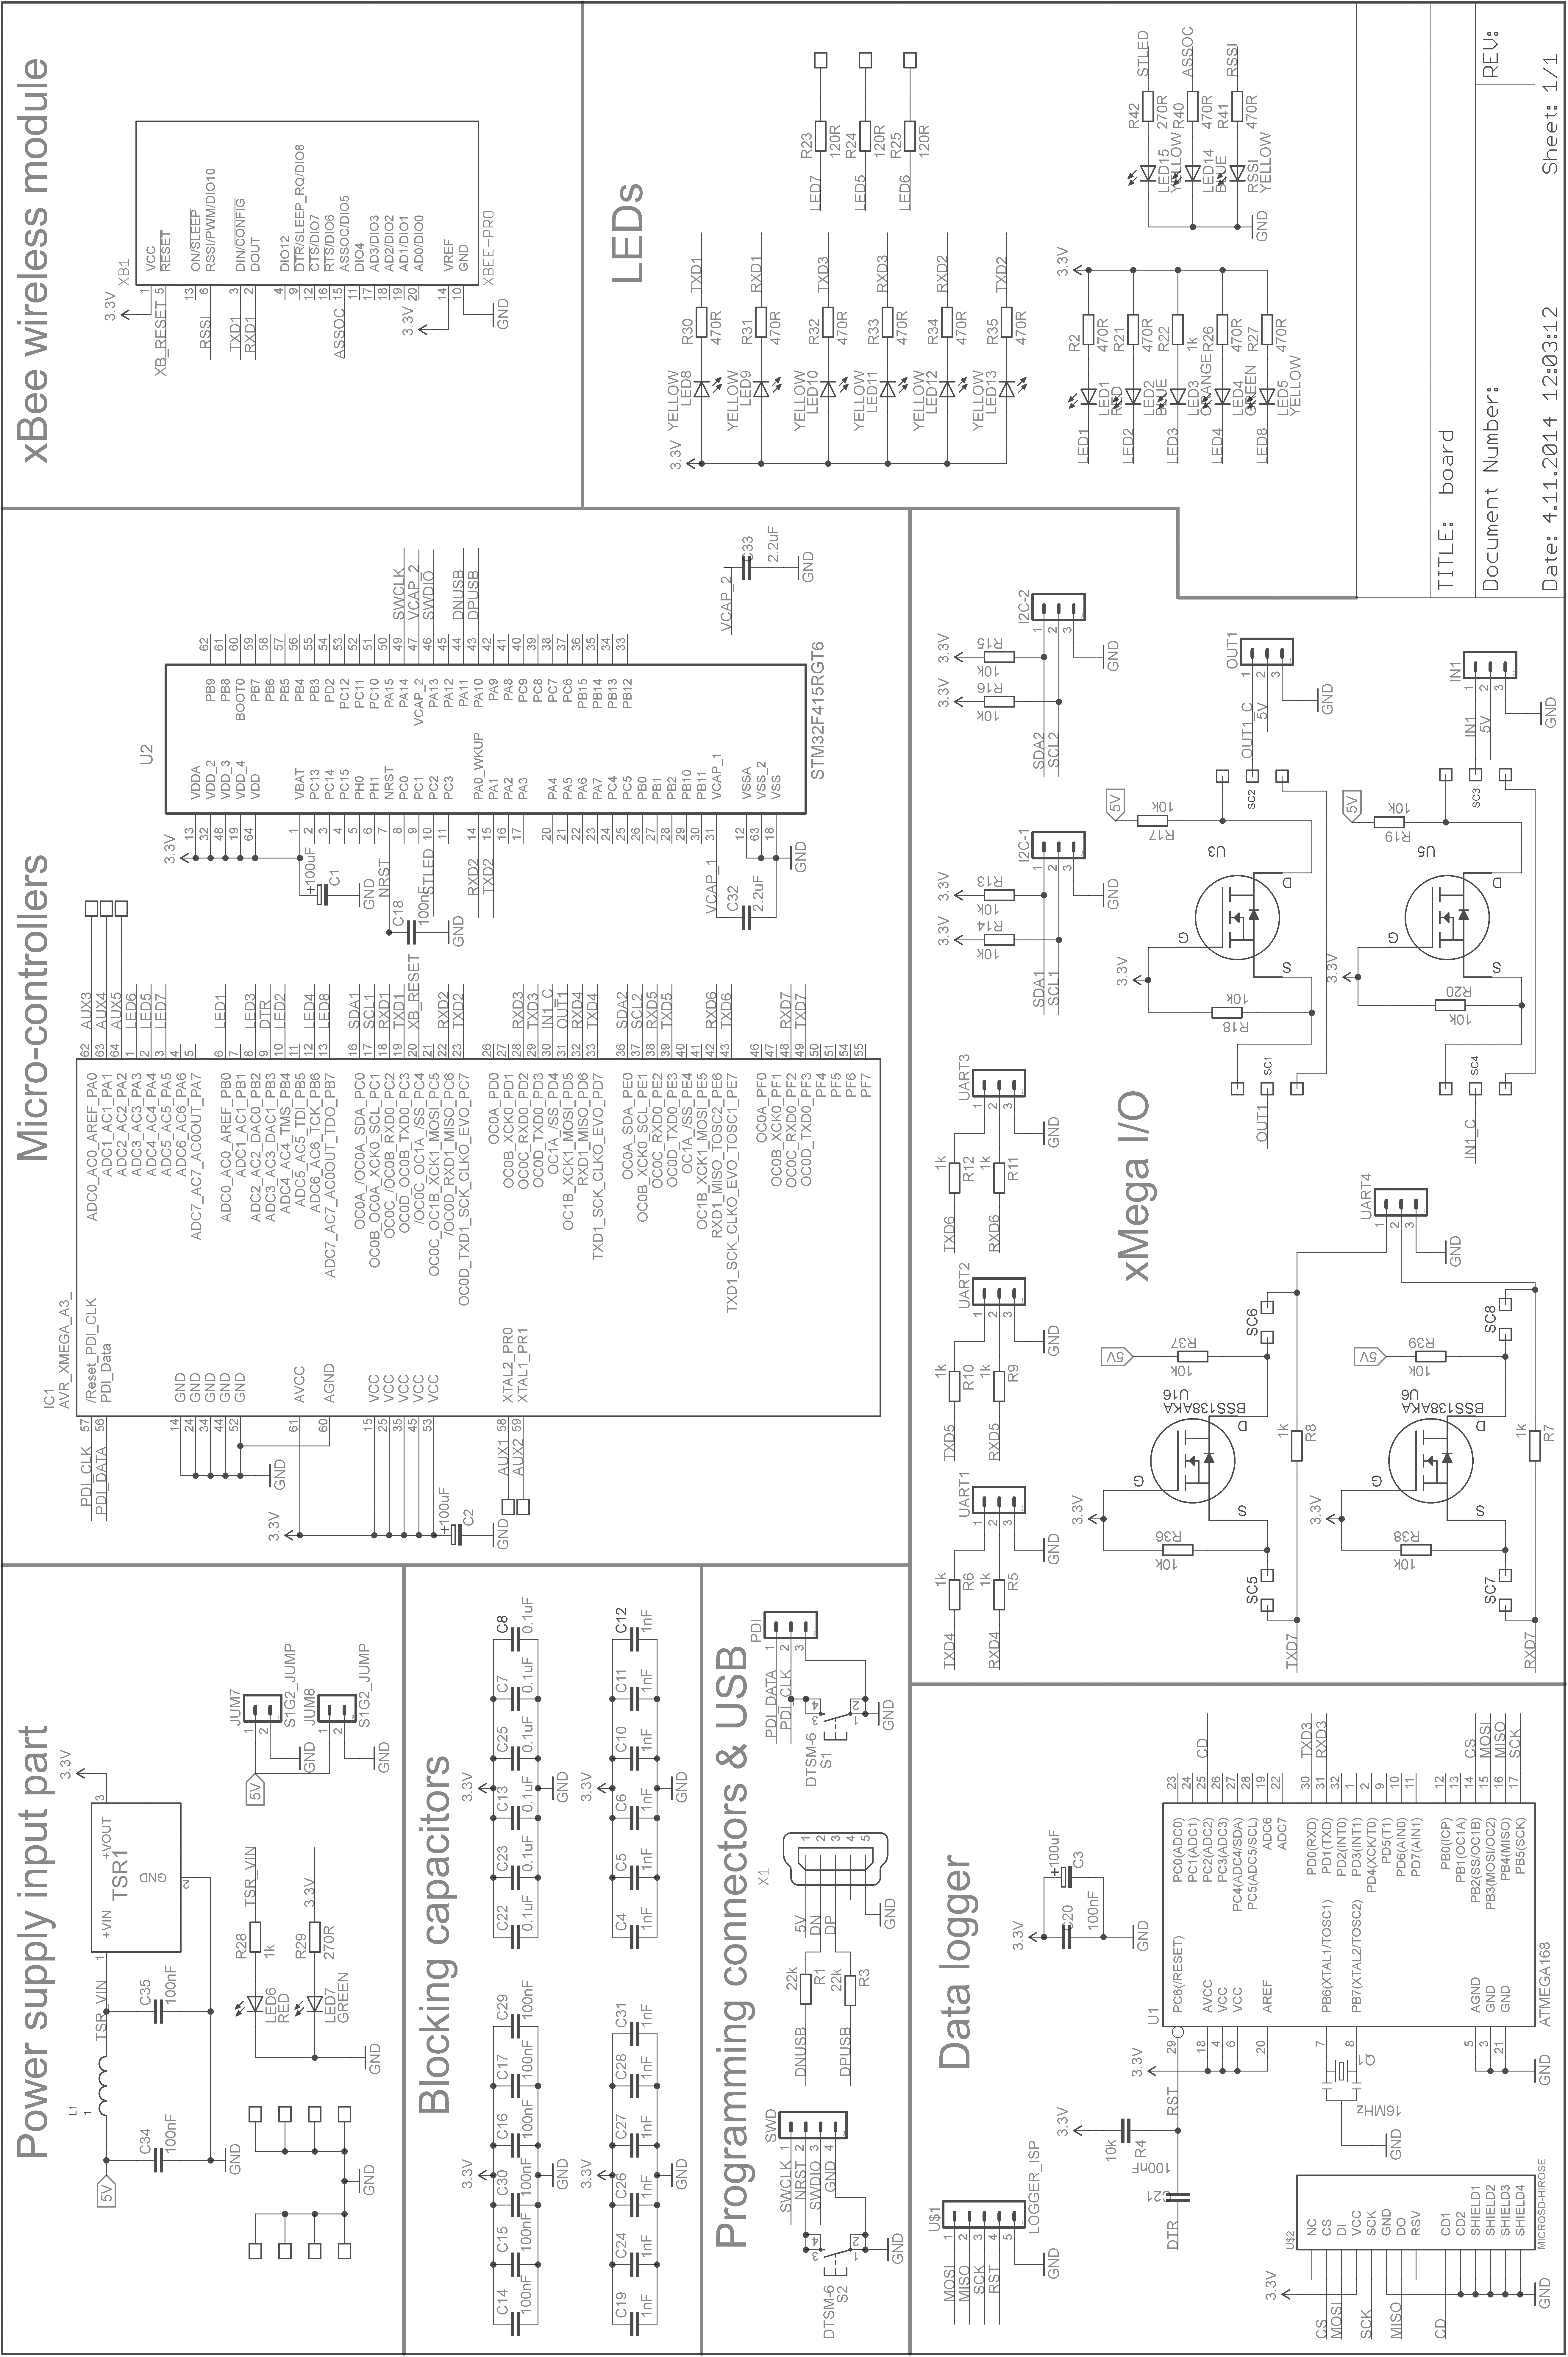
\includegraphics[width=0.88\textwidth]{fig/schema.png}
\caption*{Electrical schematic of the custom control board v.2.}
\end{figure}

\cleardoublepage

% Schema desky
\section{PCB layouts}\label{ape:pcb}
\begin{figure}[H]
\centering
\begin{subfigure}[b]{0.5\textwidth}
	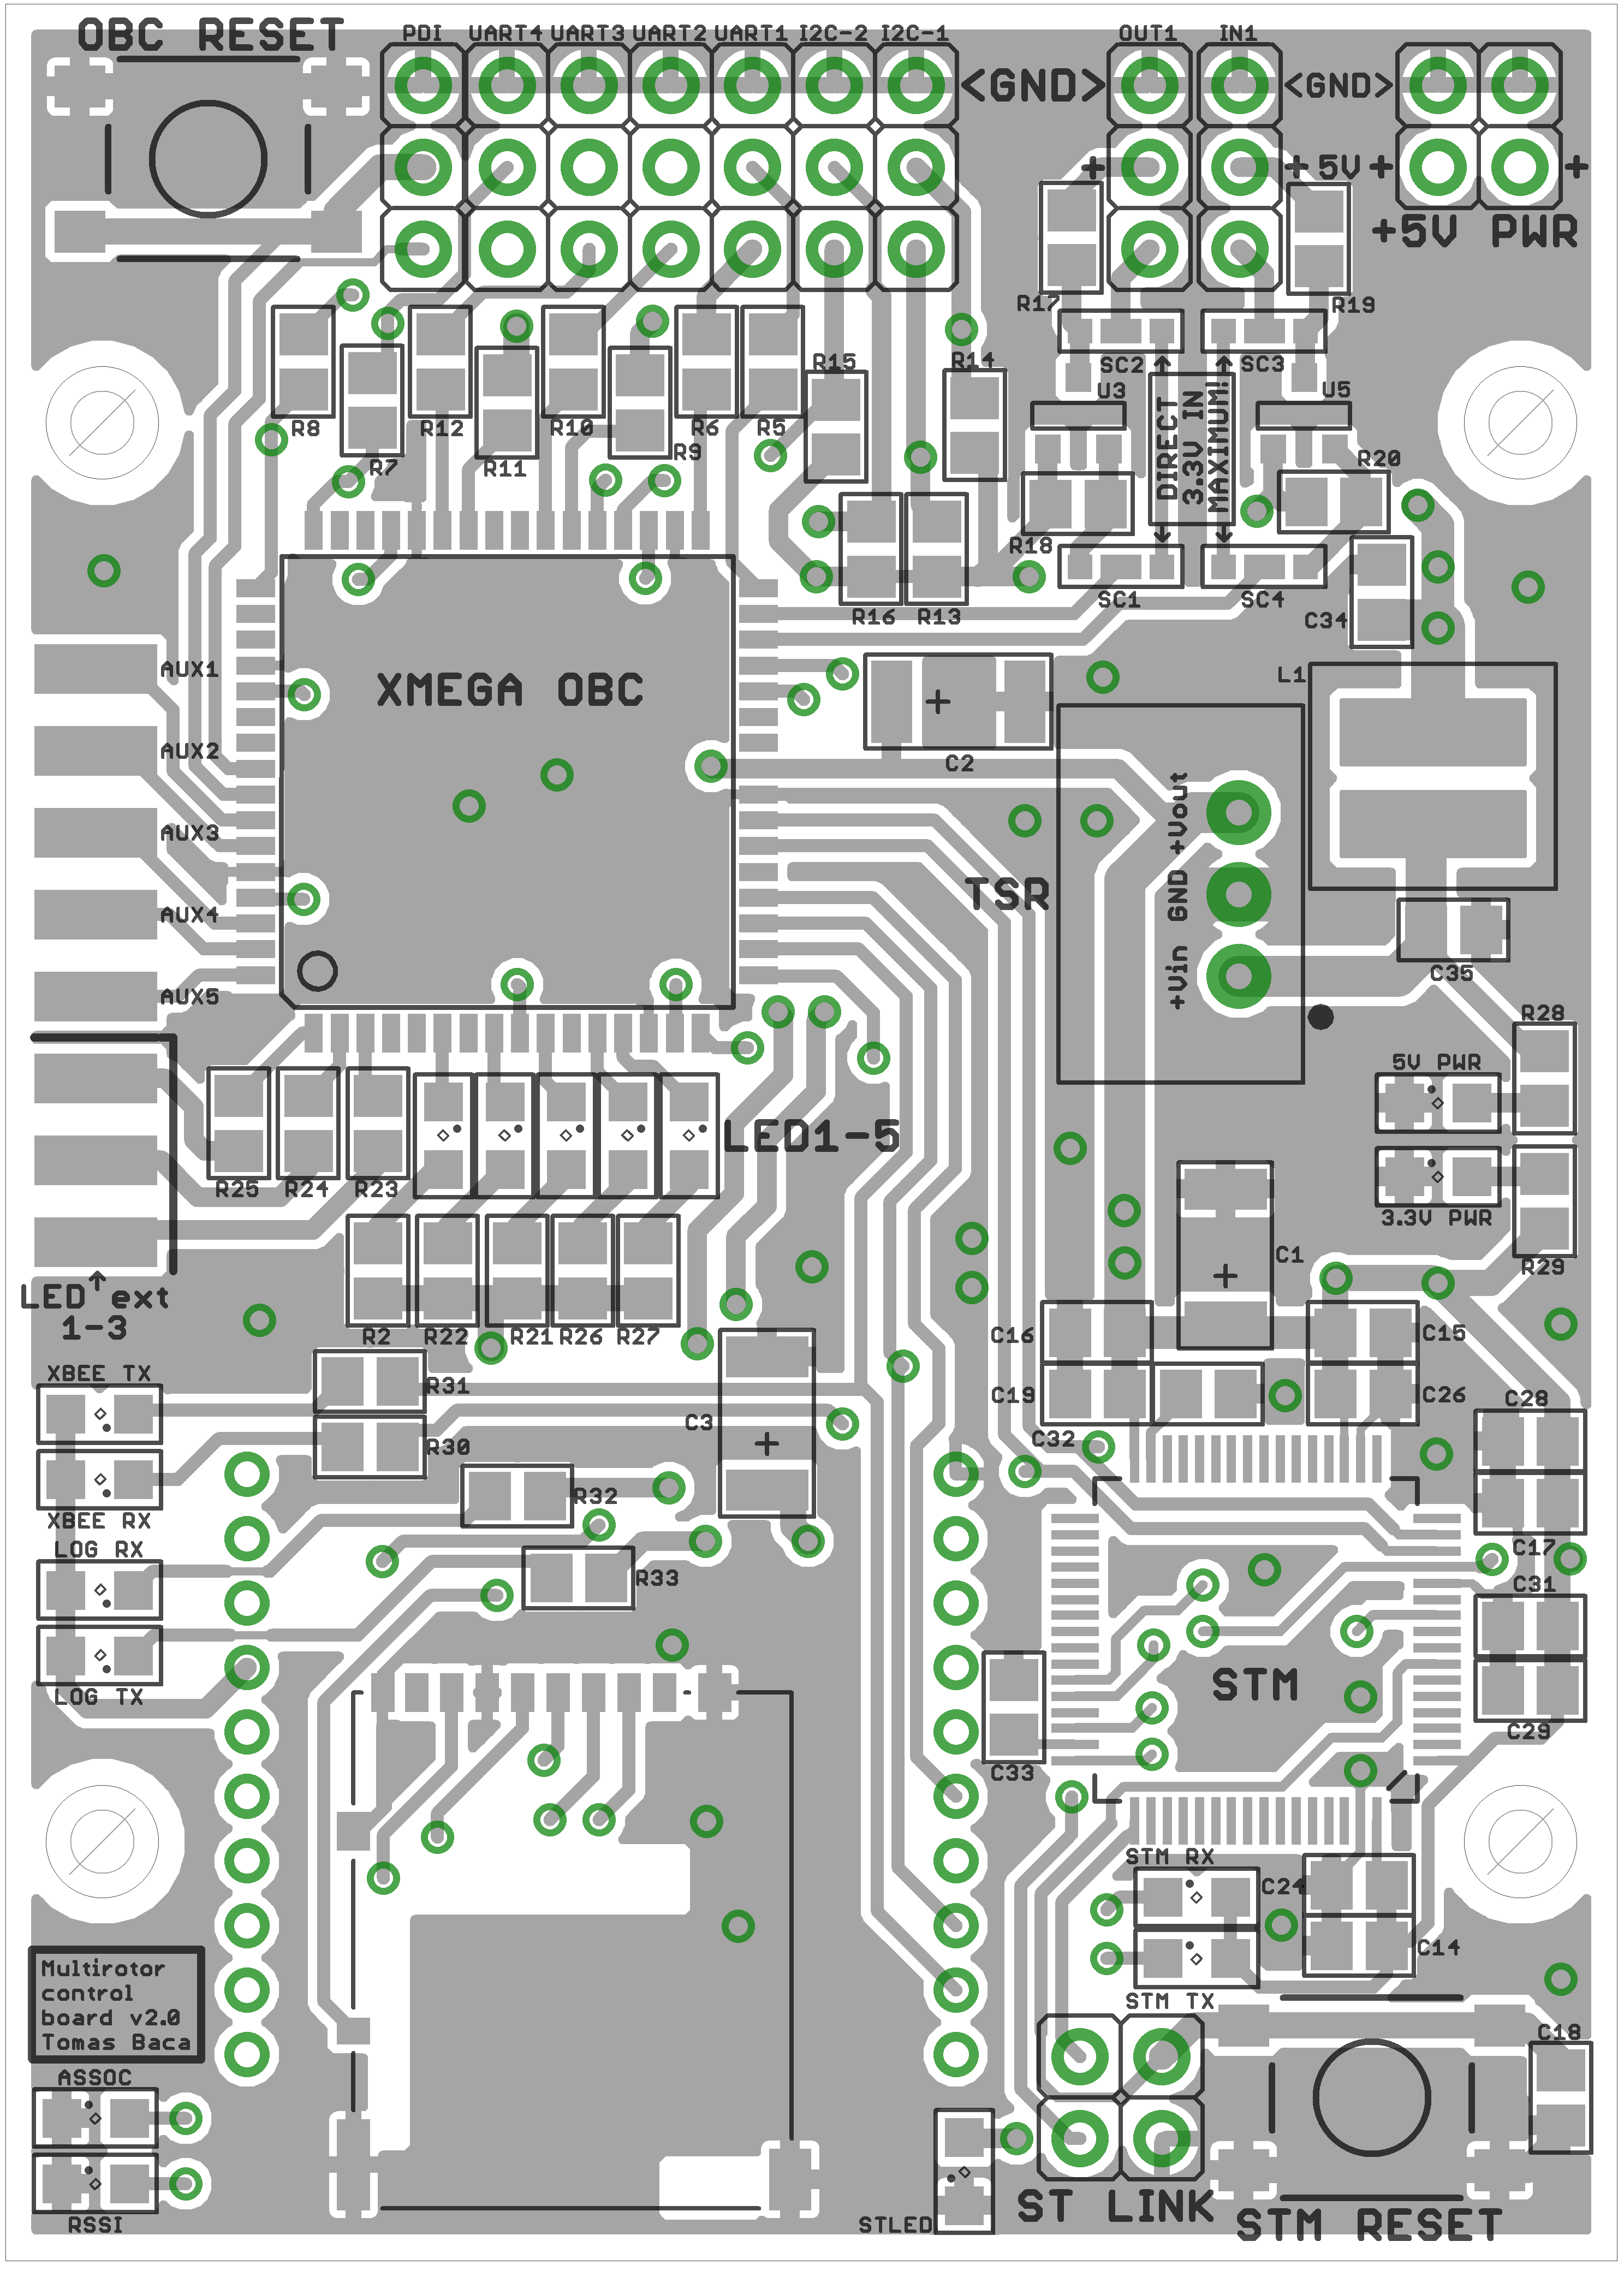
\includegraphics[width=\textwidth]{fig/layout_top.png}
	\caption{Board's top layer.}
	\label{fig:layout_top}
\end{subfigure}%
\begin{subfigure}[b]{0.5\textwidth}
	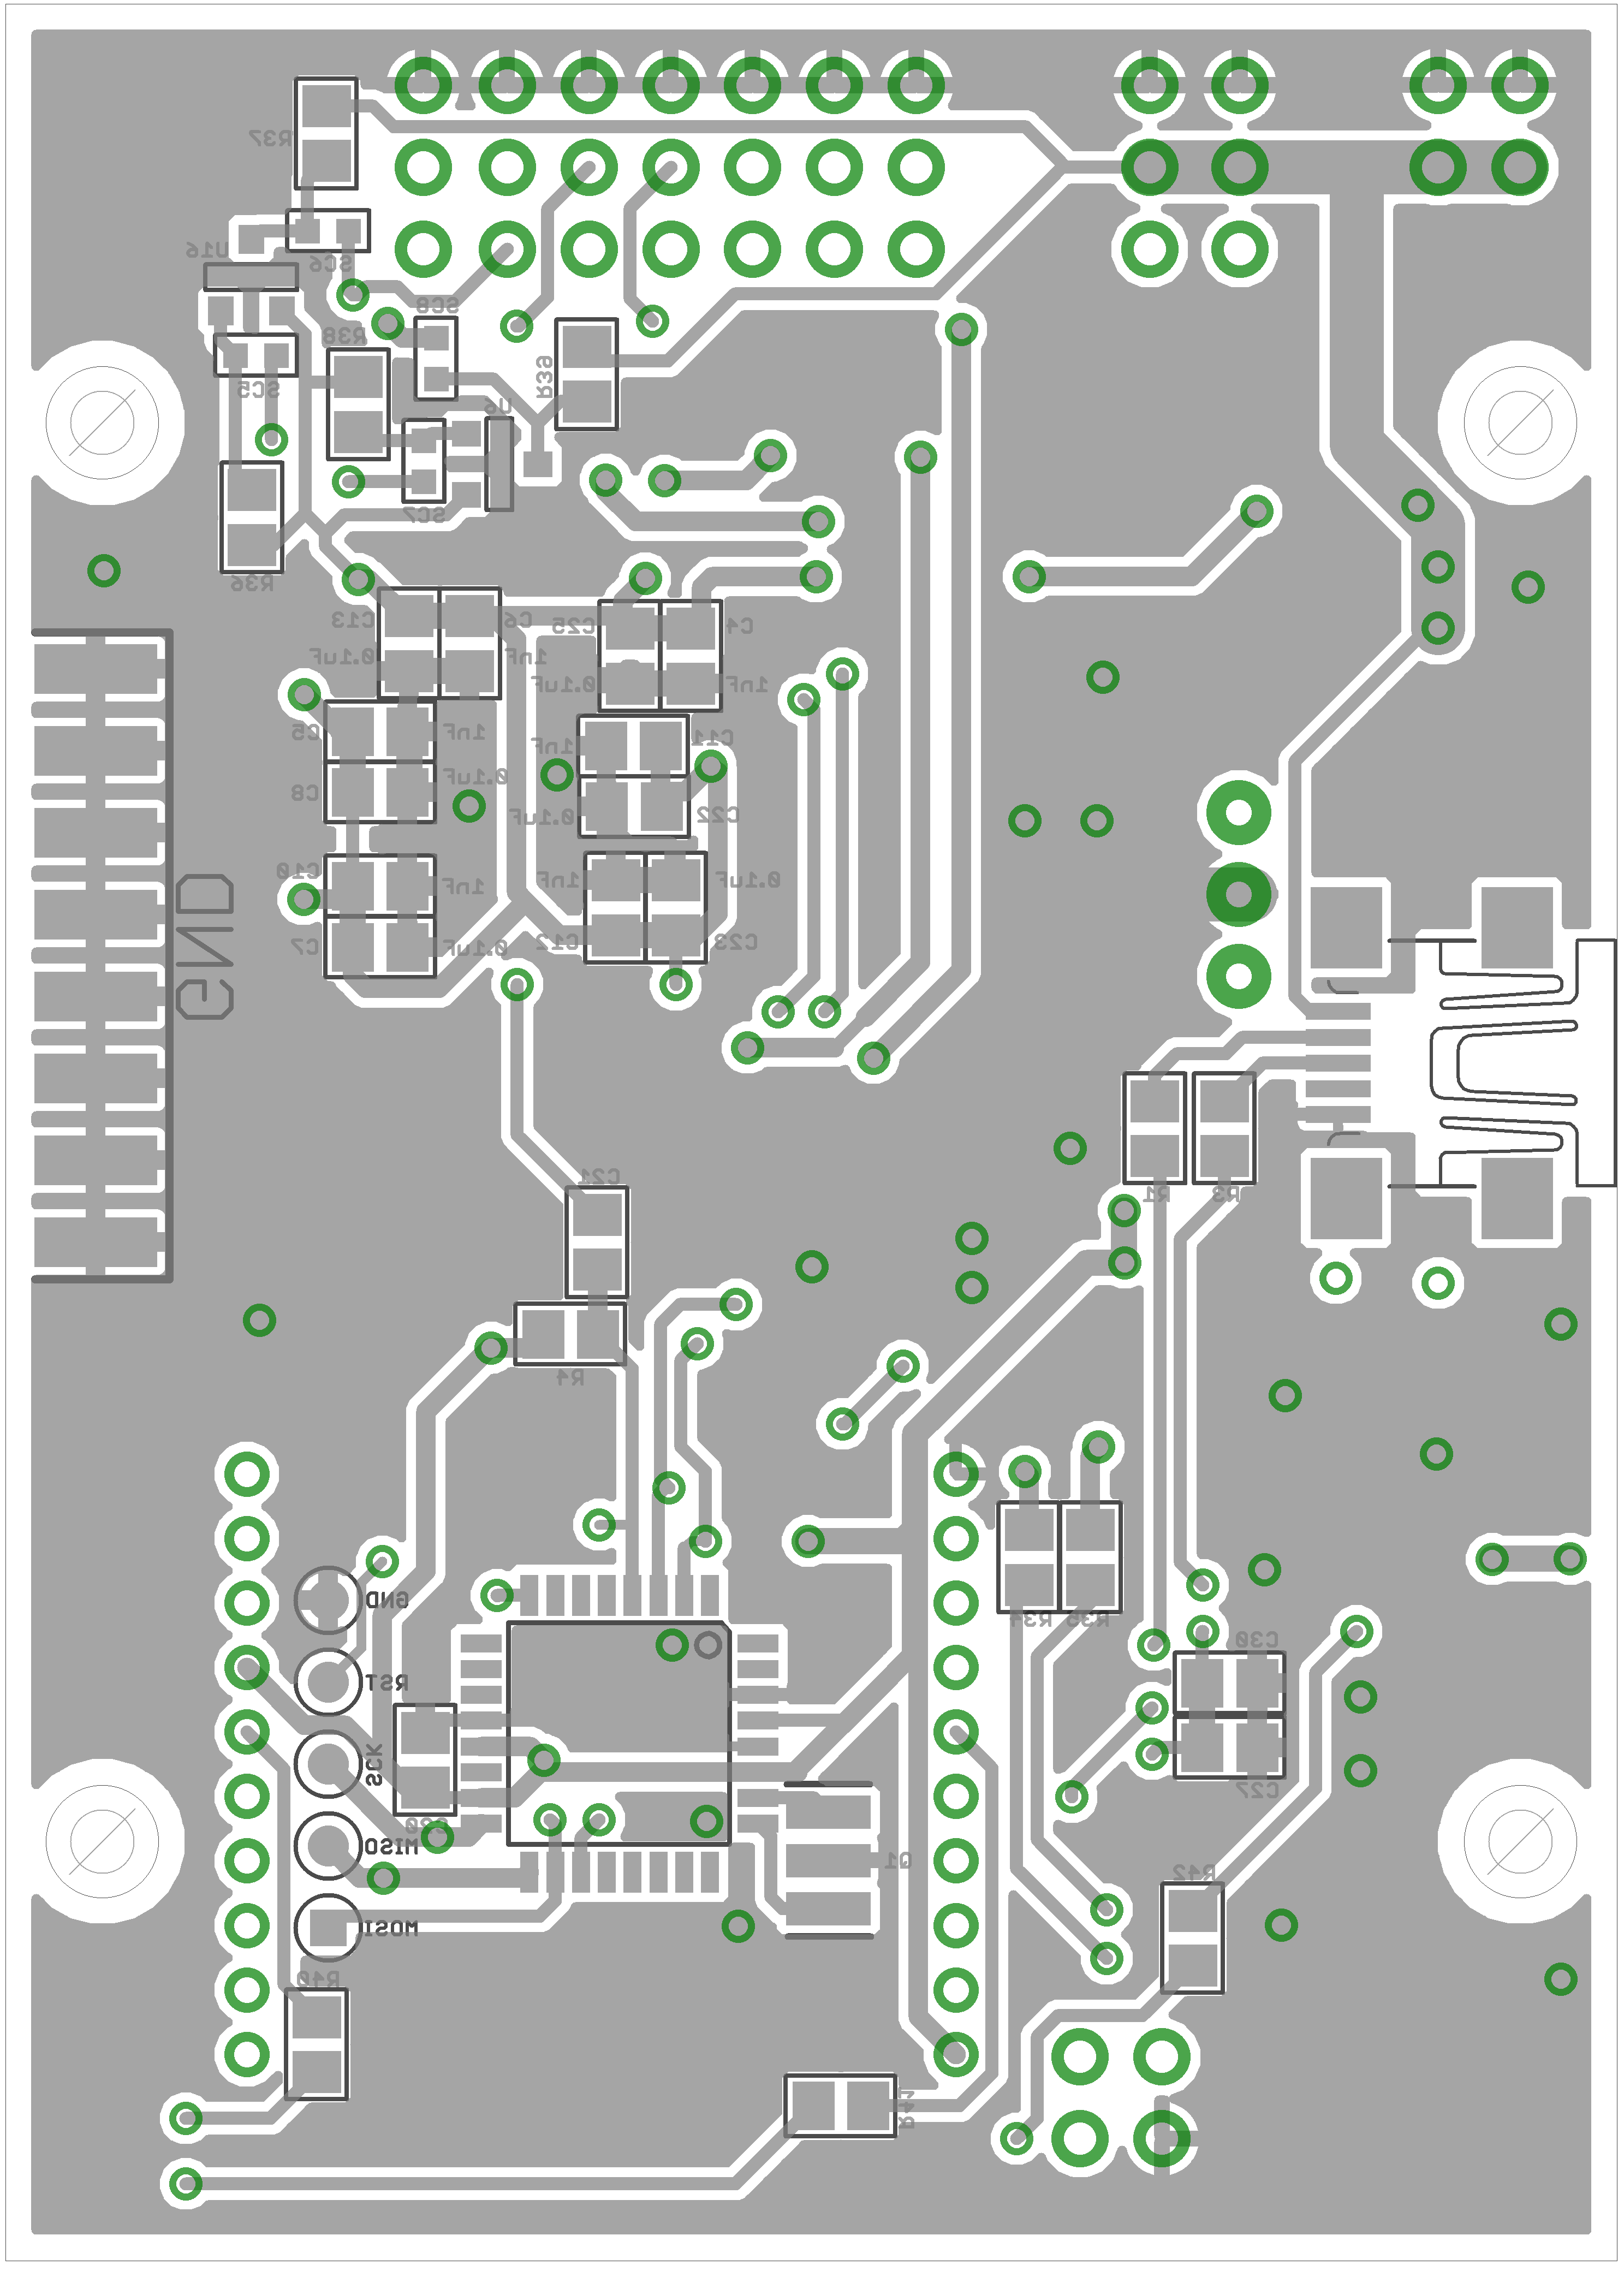
\includegraphics[width=\textwidth]{fig/layout_bottom.png}
	\caption{Board's bottom layer.}
	\label{fig:layout_bottom}
\end{subfigure}
\caption*{Printed circuit board layouts of the custom control board v.2.}
\end{figure}

\clearpage

% experiment_dlouhy_venku
\section{Additional experimental result}\label{ape:experiments}
\begin{figure}[H]
\centering
\begin{sideways}
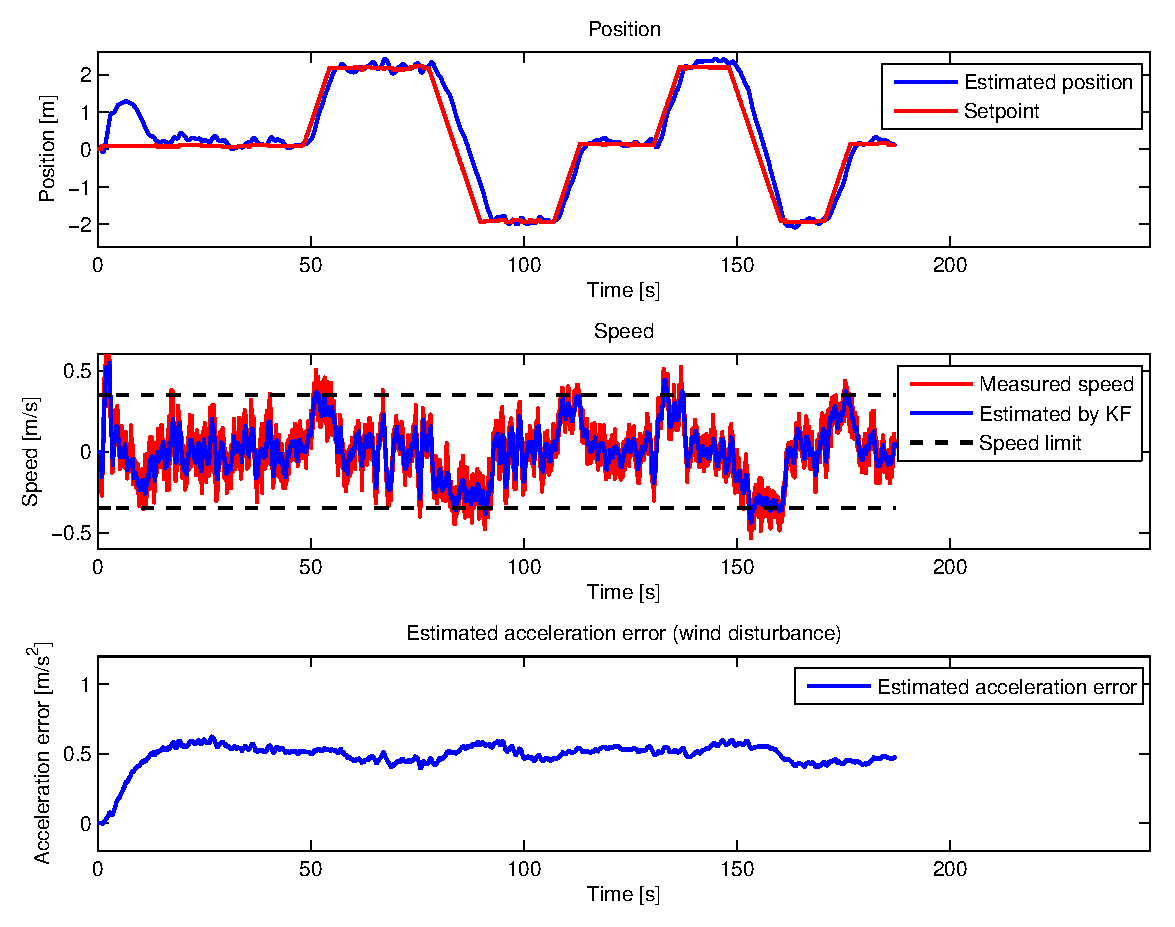
\includegraphics[scale=0.99]{fig/experiment_vitr_venku.eps}
\end{sideways}
\caption*{Data from experiment conducted during a strong wind ($5 - 10\jed{ms^{-1}}$ according to weather forecast). Notice the control lag behind the setpoint --- the desired setpoint was changing by $0.35\jed{ms^{-1}}$ which was the actual speed limit in the input governor. Since the system does not integrate the control error, there are no windup issues. Otherwise, there would be unwanted overshoots.}
\end{figure}

% experiment_dlouhy_venku
\begin{figure}[H]
\centering
\begin{sideways}
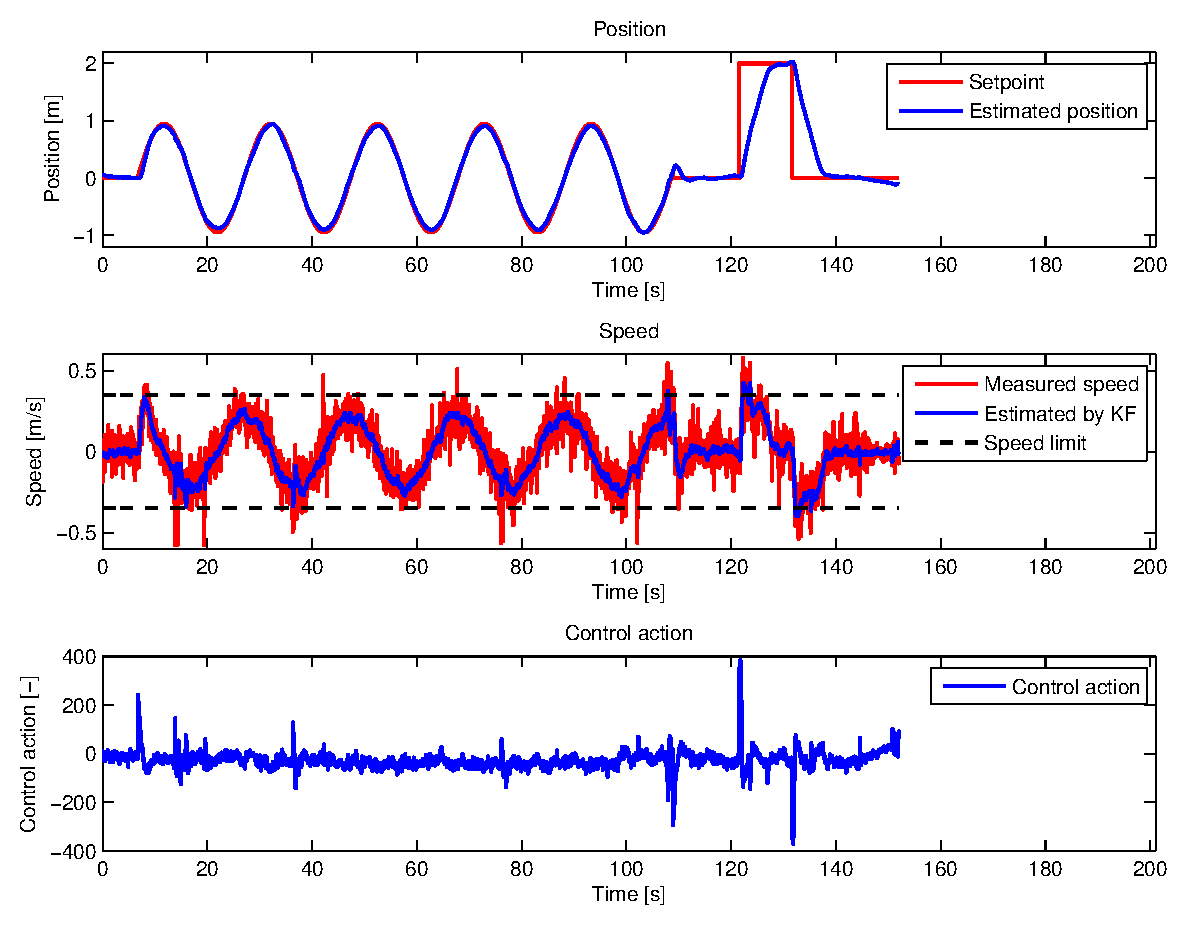
\includegraphics[scale=0.99]{fig/trajectory_circle_apendix.eps}
\end{sideways}
\caption*{blaf huhlll}
\end{figure}
